% Created by tikzDevice version 0.12.4 on 2023-07-06 14:03:29
% !TEX encoding = UTF-8 Unicode
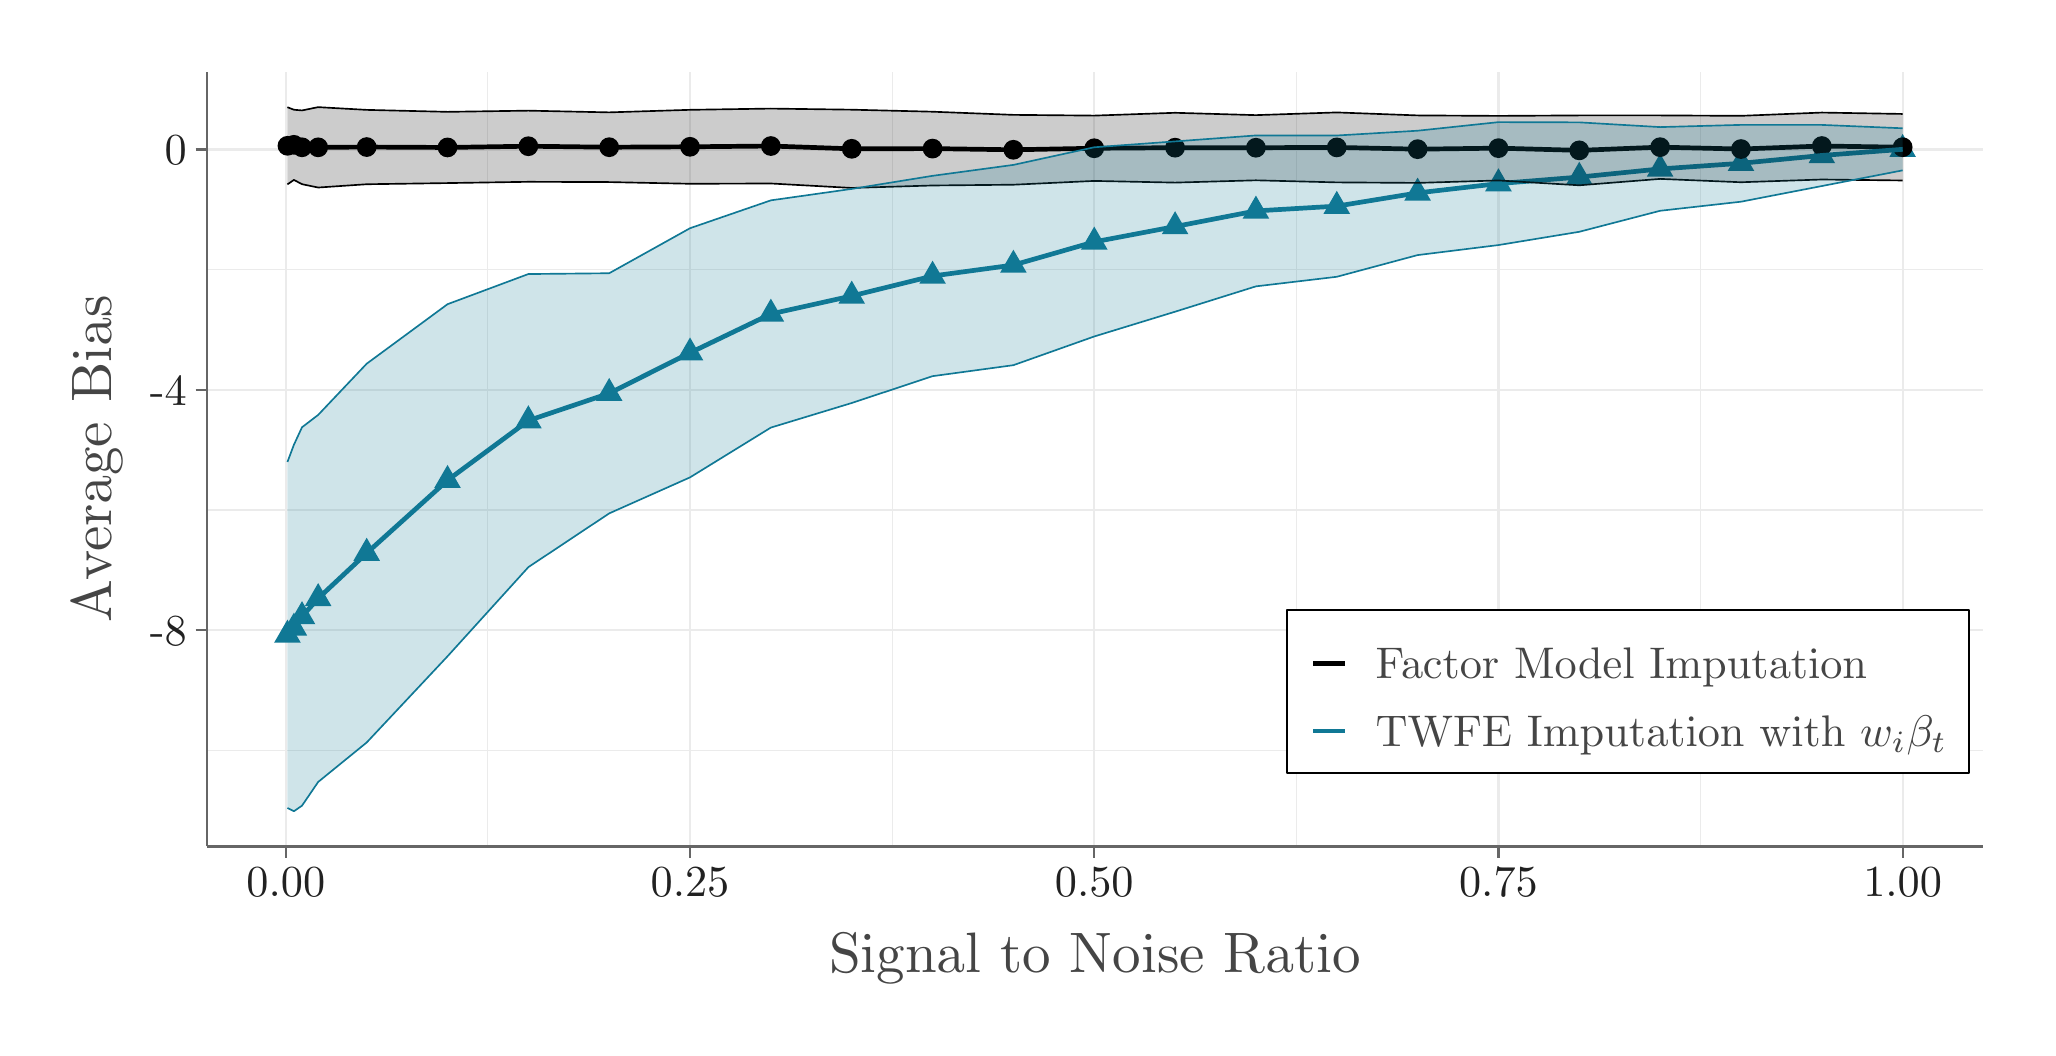
\begin{tikzpicture}[x=1pt,y=1pt]
\definecolor{fillColor}{RGB}{255,255,255}
\path[use as bounding box,fill=fillColor,fill opacity=0.00] (0,0) rectangle (722.70,361.35);
\begin{scope}
\path[clip] (  0.00,  0.00) rectangle (722.70,361.35);
\definecolor{fillColor}{RGB}{255,255,255}

\path[fill=fillColor] (  0.00,  0.00) rectangle (722.70,361.35);
\end{scope}
\begin{scope}
\path[clip] ( 64.69, 65.49) rectangle (706.70,345.35);
\definecolor{fillColor}{RGB}{255,255,255}

\path[fill=fillColor] ( 64.69, 65.49) rectangle (706.70,345.35);
\definecolor{drawColor}{gray}{0.92}

\path[draw=drawColor,line width= 0.4pt,line join=round] ( 64.69,100.20) --
	(706.70,100.20);

\path[draw=drawColor,line width= 0.4pt,line join=round] ( 64.69,187.06) --
	(706.70,187.06);

\path[draw=drawColor,line width= 0.4pt,line join=round] ( 64.69,273.91) --
	(706.70,273.91);

\path[draw=drawColor,line width= 0.4pt,line join=round] (166.31, 65.49) --
	(166.31,345.35);

\path[draw=drawColor,line width= 0.4pt,line join=round] (312.37, 65.49) --
	(312.37,345.35);

\path[draw=drawColor,line width= 0.4pt,line join=round] (458.43, 65.49) --
	(458.43,345.35);

\path[draw=drawColor,line width= 0.4pt,line join=round] (604.49, 65.49) --
	(604.49,345.35);

\path[draw=drawColor,line width= 0.8pt,line join=round] ( 64.69,143.63) --
	(706.70,143.63);

\path[draw=drawColor,line width= 0.8pt,line join=round] ( 64.69,230.49) --
	(706.70,230.49);

\path[draw=drawColor,line width= 0.8pt,line join=round] ( 64.69,317.34) --
	(706.70,317.34);

\path[draw=drawColor,line width= 0.8pt,line join=round] ( 93.29, 65.49) --
	( 93.29,345.35);

\path[draw=drawColor,line width= 0.8pt,line join=round] (239.34, 65.49) --
	(239.34,345.35);

\path[draw=drawColor,line width= 0.8pt,line join=round] (385.40, 65.49) --
	(385.40,345.35);

\path[draw=drawColor,line width= 0.8pt,line join=round] (531.46, 65.49) --
	(531.46,345.35);

\path[draw=drawColor,line width= 0.8pt,line join=round] (677.52, 65.49) --
	(677.52,345.35);
\definecolor{fillColor}{RGB}{16,120,149}

\path[fill=fillColor] ( 93.87,147.45) --
	( 98.68,139.12) --
	( 89.06,139.12) --
	cycle;

\path[fill=fillColor] ( 96.21,149.98) --
	(101.01,141.66) --
	( 91.40,141.66) --
	cycle;

\path[fill=fillColor] ( 99.13,154.13) --
	(103.93,145.81) --
	( 94.32,145.81) --
	cycle;

\path[fill=fillColor] (104.97,160.66) --
	(109.78,152.33) --
	(100.16,152.33) --
	cycle;

\path[fill=fillColor] (122.50,177.04) --
	(127.30,168.71) --
	(117.69,168.71) --
	cycle;

\path[fill=fillColor] (151.71,203.35) --
	(156.51,195.03) --
	(146.90,195.03) --
	cycle;

\path[fill=fillColor] (180.92,224.91) --
	(185.73,216.59) --
	(176.11,216.59) --
	cycle;

\path[fill=fillColor] (210.13,234.77) --
	(214.94,226.45) --
	(205.33,226.45) --
	cycle;

\path[fill=fillColor] (239.34,249.41) --
	(244.15,241.09) --
	(234.54,241.09) --
	cycle;

\path[fill=fillColor] (268.55,263.44) --
	(273.36,255.12) --
	(263.75,255.12) --
	cycle;

\path[fill=fillColor] (297.77,269.95) --
	(302.57,261.62) --
	(292.96,261.62) --
	cycle;

\path[fill=fillColor] (326.98,277.16) --
	(331.78,268.84) --
	(322.17,268.84) --
	cycle;

\path[fill=fillColor] (356.19,281.12) --
	(361.00,272.80) --
	(351.38,272.80) --
	cycle;

\path[fill=fillColor] (385.40,289.49) --
	(390.21,281.17) --
	(380.60,281.17) --
	cycle;

\path[fill=fillColor] (414.61,295.03) --
	(419.42,286.71) --
	(409.81,286.71) --
	cycle;

\path[fill=fillColor] (443.82,300.68) --
	(448.63,292.36) --
	(439.02,292.36) --
	cycle;

\path[fill=fillColor] (473.04,302.40) --
	(477.84,294.08) --
	(468.23,294.08) --
	cycle;

\path[fill=fillColor] (502.25,307.19) --
	(507.05,298.87) --
	(497.44,298.87) --
	cycle;

\path[fill=fillColor] (531.46,310.55) --
	(536.27,302.23) --
	(526.65,302.23) --
	cycle;

\path[fill=fillColor] (560.67,312.91) --
	(565.48,304.58) --
	(555.87,304.58) --
	cycle;

\path[fill=fillColor] (589.88,315.85) --
	(594.69,307.52) --
	(585.08,307.52) --
	cycle;

\path[fill=fillColor] (619.09,317.89) --
	(623.90,309.57) --
	(614.29,309.57) --
	cycle;

\path[fill=fillColor] (648.31,320.72) --
	(653.11,312.39) --
	(643.50,312.39) --
	cycle;

\path[fill=fillColor] (677.52,322.94) --
	(682.32,314.62) --
	(672.71,314.62) --
	cycle;
\definecolor{fillColor}{RGB}{0,0,0}

\path[fill=fillColor] ( 93.87,318.66) circle (  3.57);

\path[fill=fillColor] ( 96.21,319.01) circle (  3.57);

\path[fill=fillColor] ( 99.13,318.12) circle (  3.57);

\path[fill=fillColor] (104.97,318.11) circle (  3.57);

\path[fill=fillColor] (122.50,318.21) circle (  3.57);

\path[fill=fillColor] (151.71,318.06) circle (  3.57);

\path[fill=fillColor] (180.92,318.51) circle (  3.57);

\path[fill=fillColor] (210.13,318.15) circle (  3.57);

\path[fill=fillColor] (239.34,318.30) circle (  3.57);

\path[fill=fillColor] (268.55,318.58) circle (  3.57);

\path[fill=fillColor] (297.77,317.57) circle (  3.57);

\path[fill=fillColor] (326.98,317.65) circle (  3.57);

\path[fill=fillColor] (356.19,317.22) circle (  3.57);

\path[fill=fillColor] (385.40,317.77) circle (  3.57);

\path[fill=fillColor] (414.61,317.98) circle (  3.57);

\path[fill=fillColor] (443.82,317.97) circle (  3.57);

\path[fill=fillColor] (473.04,318.08) circle (  3.57);

\path[fill=fillColor] (502.25,317.44) circle (  3.57);

\path[fill=fillColor] (531.46,317.81) circle (  3.57);

\path[fill=fillColor] (560.67,317.01) circle (  3.57);

\path[fill=fillColor] (589.88,318.17) circle (  3.57);

\path[fill=fillColor] (619.09,317.49) circle (  3.57);

\path[fill=fillColor] (648.31,318.58) circle (  3.57);

\path[fill=fillColor] (677.52,318.15) circle (  3.57);
\definecolor{drawColor}{RGB}{0,0,0}

\path[draw=drawColor,line width= 1.7pt,line join=round] ( 93.87,318.66) --
	( 96.21,319.01) --
	( 99.13,318.12) --
	(104.97,318.11) --
	(122.50,318.21) --
	(151.71,318.06) --
	(180.92,318.51) --
	(210.13,318.15) --
	(239.34,318.30) --
	(268.55,318.58) --
	(297.77,317.57) --
	(326.98,317.65) --
	(356.19,317.22) --
	(385.40,317.77) --
	(414.61,317.98) --
	(443.82,317.97) --
	(473.04,318.08) --
	(502.25,317.44) --
	(531.46,317.81) --
	(560.67,317.01) --
	(589.88,318.17) --
	(619.09,317.49) --
	(648.31,318.58) --
	(677.52,318.15);
\definecolor{drawColor}{RGB}{16,120,149}

\path[draw=drawColor,line width= 1.7pt,line join=round] ( 93.87,141.90) --
	( 96.21,144.43) --
	( 99.13,148.58) --
	(104.97,155.11) --
	(122.50,171.49) --
	(151.71,197.80) --
	(180.92,219.37) --
	(210.13,229.22) --
	(239.34,243.86) --
	(268.55,257.90) --
	(297.77,264.40) --
	(326.98,271.61) --
	(356.19,275.57) --
	(385.40,283.94) --
	(414.61,289.48) --
	(443.82,295.13) --
	(473.04,296.86) --
	(502.25,301.64) --
	(531.46,305.00) --
	(560.67,307.36) --
	(589.88,310.30) --
	(619.09,312.34) --
	(648.31,315.17) --
	(677.52,317.39);
\definecolor{fillColor}{RGB}{0,0,0}

\path[fill=fillColor,fill opacity=0.20] ( 93.87,332.60) --
	( 96.21,331.69) --
	( 99.13,331.44) --
	(104.97,332.63) --
	(122.50,331.64) --
	(151.71,330.93) --
	(180.92,331.36) --
	(210.13,330.74) --
	(239.34,331.66) --
	(268.55,332.11) --
	(297.77,331.71) --
	(326.98,330.98) --
	(356.19,329.84) --
	(385.40,329.57) --
	(414.61,330.59) --
	(443.82,329.74) --
	(473.04,330.72) --
	(502.25,329.64) --
	(531.46,329.47) --
	(560.67,329.64) --
	(589.88,329.64) --
	(619.09,329.49) --
	(648.31,330.67) --
	(677.52,330.17) --
	(677.52,306.13) --
	(648.31,306.48) --
	(619.09,305.49) --
	(589.88,306.70) --
	(560.67,304.39) --
	(531.46,306.14) --
	(502.25,305.25) --
	(473.04,305.44) --
	(443.82,306.19) --
	(414.61,305.36) --
	(385.40,305.97) --
	(356.19,304.60) --
	(326.98,304.32) --
	(297.77,303.43) --
	(268.55,305.04) --
	(239.34,304.94) --
	(210.13,305.55) --
	(180.92,305.65) --
	(151.71,305.19) --
	(122.50,304.77) --
	(104.97,303.58) --
	( 99.13,304.79) --
	( 96.21,306.33) --
	( 93.87,304.73) --
	cycle;
\definecolor{drawColor}{RGB}{0,0,0}

\path[draw=drawColor,line width= 0.6pt,line join=round] ( 93.87,332.60) --
	( 96.21,331.69) --
	( 99.13,331.44) --
	(104.97,332.63) --
	(122.50,331.64) --
	(151.71,330.93) --
	(180.92,331.36) --
	(210.13,330.74) --
	(239.34,331.66) --
	(268.55,332.11) --
	(297.77,331.71) --
	(326.98,330.98) --
	(356.19,329.84) --
	(385.40,329.57) --
	(414.61,330.59) --
	(443.82,329.74) --
	(473.04,330.72) --
	(502.25,329.64) --
	(531.46,329.47) --
	(560.67,329.64) --
	(589.88,329.64) --
	(619.09,329.49) --
	(648.31,330.67) --
	(677.52,330.17);

\path[draw=drawColor,line width= 0.6pt,line join=round] (677.52,306.13) --
	(648.31,306.48) --
	(619.09,305.49) --
	(589.88,306.70) --
	(560.67,304.39) --
	(531.46,306.14) --
	(502.25,305.25) --
	(473.04,305.44) --
	(443.82,306.19) --
	(414.61,305.36) --
	(385.40,305.97) --
	(356.19,304.60) --
	(326.98,304.32) --
	(297.77,303.43) --
	(268.55,305.04) --
	(239.34,304.94) --
	(210.13,305.55) --
	(180.92,305.65) --
	(151.71,305.19) --
	(122.50,304.77) --
	(104.97,303.58) --
	( 99.13,304.79) --
	( 96.21,306.33) --
	( 93.87,304.73);
\definecolor{fillColor}{RGB}{16,120,149}

\path[fill=fillColor,fill opacity=0.20] ( 93.87,204.42) --
	( 96.21,210.65) --
	( 99.13,216.95) --
	(104.97,221.42) --
	(122.50,239.92) --
	(151.71,261.42) --
	(180.92,272.32) --
	(210.13,272.61) --
	(239.34,288.88) --
	(268.55,298.95) --
	(297.77,303.08) --
	(326.98,307.81) --
	(356.19,311.76) --
	(385.40,318.13) --
	(414.61,320.25) --
	(443.82,322.40) --
	(473.04,322.38) --
	(502.25,324.11) --
	(531.46,327.21) --
	(560.67,327.13) --
	(589.88,325.42) --
	(619.09,326.22) --
	(648.31,326.21) --
	(677.52,324.99) --
	(677.52,309.79) --
	(648.31,304.12) --
	(619.09,298.46) --
	(589.88,295.18) --
	(560.67,287.59) --
	(531.46,282.79) --
	(502.25,279.17) --
	(473.04,271.33) --
	(443.82,267.87) --
	(414.61,258.71) --
	(385.40,249.76) --
	(356.19,239.39) --
	(326.98,235.42) --
	(297.77,225.72) --
	(268.55,216.84) --
	(239.34,198.85) --
	(210.13,185.83) --
	(180.92,166.41) --
	(151.71,134.19) --
	(122.50,103.05) --
	(104.97, 88.79) --
	( 99.13, 80.22) --
	( 96.21, 78.21) --
	( 93.87, 79.38) --
	cycle;
\definecolor{drawColor}{RGB}{16,120,149}

\path[draw=drawColor,line width= 0.6pt,line join=round] ( 93.87,204.42) --
	( 96.21,210.65) --
	( 99.13,216.95) --
	(104.97,221.42) --
	(122.50,239.92) --
	(151.71,261.42) --
	(180.92,272.32) --
	(210.13,272.61) --
	(239.34,288.88) --
	(268.55,298.95) --
	(297.77,303.08) --
	(326.98,307.81) --
	(356.19,311.76) --
	(385.40,318.13) --
	(414.61,320.25) --
	(443.82,322.40) --
	(473.04,322.38) --
	(502.25,324.11) --
	(531.46,327.21) --
	(560.67,327.13) --
	(589.88,325.42) --
	(619.09,326.22) --
	(648.31,326.21) --
	(677.52,324.99);

\path[draw=drawColor,line width= 0.6pt,line join=round] (677.52,309.79) --
	(648.31,304.12) --
	(619.09,298.46) --
	(589.88,295.18) --
	(560.67,287.59) --
	(531.46,282.79) --
	(502.25,279.17) --
	(473.04,271.33) --
	(443.82,267.87) --
	(414.61,258.71) --
	(385.40,249.76) --
	(356.19,239.39) --
	(326.98,235.42) --
	(297.77,225.72) --
	(268.55,216.84) --
	(239.34,198.85) --
	(210.13,185.83) --
	(180.92,166.41) --
	(151.71,134.19) --
	(122.50,103.05) --
	(104.97, 88.79) --
	( 99.13, 80.22) --
	( 96.21, 78.21) --
	( 93.87, 79.38);

\path[] ( 64.69, 65.49) rectangle (706.70,345.35);
\end{scope}
\begin{scope}
\path[clip] (  0.00,  0.00) rectangle (722.70,361.35);
\definecolor{drawColor}{gray}{0.40}

\path[draw=drawColor,line width= 0.8pt,line join=round] ( 64.69, 65.49) --
	( 64.69,345.35);
\end{scope}
\begin{scope}
\path[clip] (  0.00,  0.00) rectangle (722.70,361.35);
\definecolor{drawColor}{gray}{0.13}

\node[text=drawColor,anchor=base east,inner sep=0pt, outer sep=0pt, scale=  1.60] at ( 57.49,138.12) {-8};

\node[text=drawColor,anchor=base east,inner sep=0pt, outer sep=0pt, scale=  1.60] at ( 57.49,224.98) {-4};

\node[text=drawColor,anchor=base east,inner sep=0pt, outer sep=0pt, scale=  1.60] at ( 57.49,311.83) {0};
\end{scope}
\begin{scope}
\path[clip] (  0.00,  0.00) rectangle (722.70,361.35);
\definecolor{drawColor}{gray}{0.40}

\path[draw=drawColor,line width= 0.8pt,line join=round] ( 60.69,143.63) --
	( 64.69,143.63);

\path[draw=drawColor,line width= 0.8pt,line join=round] ( 60.69,230.49) --
	( 64.69,230.49);

\path[draw=drawColor,line width= 0.8pt,line join=round] ( 60.69,317.34) --
	( 64.69,317.34);
\end{scope}
\begin{scope}
\path[clip] (  0.00,  0.00) rectangle (722.70,361.35);
\definecolor{drawColor}{gray}{0.40}

\path[draw=drawColor,line width= 0.8pt,line join=round] ( 64.69, 65.49) --
	(706.70, 65.49);
\end{scope}
\begin{scope}
\path[clip] (  0.00,  0.00) rectangle (722.70,361.35);
\definecolor{drawColor}{gray}{0.40}

\path[draw=drawColor,line width= 0.8pt,line join=round] ( 93.29, 61.49) --
	( 93.29, 65.49);

\path[draw=drawColor,line width= 0.8pt,line join=round] (239.34, 61.49) --
	(239.34, 65.49);

\path[draw=drawColor,line width= 0.8pt,line join=round] (385.40, 61.49) --
	(385.40, 65.49);

\path[draw=drawColor,line width= 0.8pt,line join=round] (531.46, 61.49) --
	(531.46, 65.49);

\path[draw=drawColor,line width= 0.8pt,line join=round] (677.52, 61.49) --
	(677.52, 65.49);
\end{scope}
\begin{scope}
\path[clip] (  0.00,  0.00) rectangle (722.70,361.35);
\definecolor{drawColor}{gray}{0.13}

\node[text=drawColor,anchor=base,inner sep=0pt, outer sep=0pt, scale=  1.60] at ( 93.29, 47.27) {0.00};

\node[text=drawColor,anchor=base,inner sep=0pt, outer sep=0pt, scale=  1.60] at (239.34, 47.27) {0.25};

\node[text=drawColor,anchor=base,inner sep=0pt, outer sep=0pt, scale=  1.60] at (385.40, 47.27) {0.50};

\node[text=drawColor,anchor=base,inner sep=0pt, outer sep=0pt, scale=  1.60] at (531.46, 47.27) {0.75};

\node[text=drawColor,anchor=base,inner sep=0pt, outer sep=0pt, scale=  1.60] at (677.52, 47.27) {1.00};
\end{scope}
\begin{scope}
\path[clip] (  0.00,  0.00) rectangle (722.70,361.35);
\definecolor{drawColor}{gray}{0.27}

\node[text=drawColor,anchor=base,inner sep=0pt, outer sep=0pt, scale=  2.06] at (385.69, 20.00) {Signal to Noise Ratio};
\end{scope}
\begin{scope}
\path[clip] (  0.00,  0.00) rectangle (722.70,361.35);
\definecolor{drawColor}{gray}{0.27}

\node[text=drawColor,rotate= 90.00,anchor=base,inner sep=0pt, outer sep=0pt, scale=  2.06] at ( 30.16,205.42) {Average Bias};
\end{scope}
\begin{scope}
\path[clip] (  0.00,  0.00) rectangle (722.70,361.35);
\definecolor{drawColor}{RGB}{0,0,0}
\definecolor{fillColor}{RGB}{255,255,255}

\path[draw=drawColor,line width= 0.6pt,line join=round,line cap=round,fill=fillColor] (455.00, 92.01) rectangle (701.59,150.91);
\end{scope}
\begin{scope}
\path[clip] (  0.00,  0.00) rectangle (722.70,361.35);
\definecolor{fillColor}{RGB}{255,255,255}

\path[fill=fillColor] (463.00,124.46) rectangle (477.46,138.91);
\end{scope}
\begin{scope}
\path[clip] (  0.00,  0.00) rectangle (722.70,361.35);
\definecolor{fillColor}{RGB}{0,0,0}

\path[fill=fillColor] (470.23,131.69) circle (  0.36);
\end{scope}
\begin{scope}
\path[clip] (  0.00,  0.00) rectangle (722.70,361.35);
\definecolor{drawColor}{RGB}{0,0,0}

\path[draw=drawColor,line width= 1.7pt,line join=round] (464.45,131.69) -- (476.01,131.69);
\end{scope}
\begin{scope}
\path[clip] (  0.00,  0.00) rectangle (722.70,361.35);
\definecolor{fillColor}{RGB}{255,255,255}

\path[fill=fillColor] (463.00,100.01) rectangle (477.46,114.46);
\end{scope}
\begin{scope}
\path[clip] (  0.00,  0.00) rectangle (722.70,361.35);
\definecolor{fillColor}{RGB}{16,120,149}

\path[fill=fillColor] (470.23,107.79) --
	(470.71,106.96) --
	(469.75,106.96) --
	cycle;
\end{scope}
\begin{scope}
\path[clip] (  0.00,  0.00) rectangle (722.70,361.35);
\definecolor{drawColor}{RGB}{16,120,149}

\path[draw=drawColor,line width= 1.7pt,line join=round] (464.45,107.23) -- (476.01,107.23);
\end{scope}
\begin{scope}
\path[clip] (  0.00,  0.00) rectangle (722.70,361.35);
\definecolor{drawColor}{gray}{0.27}

\node[text=drawColor,anchor=base west,inner sep=0pt, outer sep=0pt, scale=  1.60] at (487.06,126.18) {Factor Model Imputation};
\end{scope}
\begin{scope}
\path[clip] (  0.00,  0.00) rectangle (722.70,361.35);
\definecolor{drawColor}{gray}{0.27}

\node[text=drawColor,anchor=base west,inner sep=0pt, outer sep=0pt, scale=  1.60] at (487.06,101.72) {TWFE Imputation with $w_i \beta_t$};
\end{scope}
\end{tikzpicture}
